\documentclass[10pt, pdf, hyperref={unicode}]{beamer}
\usetheme{metropolis} 

\usepackage{polyglossia}
\setdefaultlanguage[spelling=modern]{russian}

\usepackage{caption}
\captionsetup[figure]{labelformat=empty, font=scriptsize}
\captionsetup[table]{labelformat=empty, font=scriptsize}

\usepackage{bibentry}
\nobibliography*

\setbeamercolor{background canvas}{bg=white}
%\setbeamerfont{bibliography item}{size=\tiny}
%\setbeamerfont{bibliography entry author}{size=\tiny}
%\setbeamerfont{bibliography entry title}{size=\tiny}
%\setbeamerfont{bibliography entry location}{size=\tiny}
%\setbeamerfont{bibliography entry note}{size=\tiny}

\usepackage{subcaption}

\title{Оптический отклик Ми-резонансных наночастиц, связанных с диэлектрическими волноводами}
\date{}
\author{Нестеров~К.\,Е.}
\institute{
	МОСКОВСКИЙ ГОСУДАРСТВЕННЫЙ УНИВЕРСИТЕТ имени М.В.ЛОМОНОСОВА \\
	ФИЗИЧЕСКИЙ ФАКУЛЬТЕТ МГУ \\
	Кафедра квантовой электроники
}

\begin{document}
  	\maketitle
  
  	\begin{frame}{Оптические метаматериалы}
    \begin{minipage}[b]{.5\textwidth}
    	Неметаллические
    	\begin{figure}
    		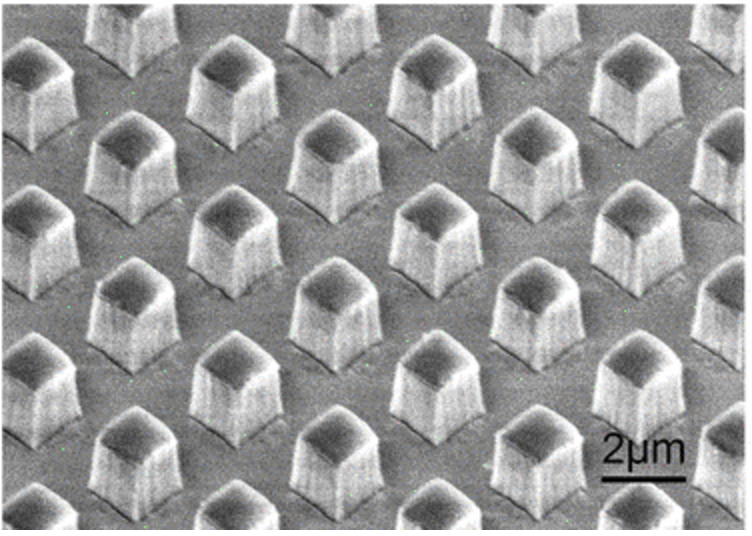
\includegraphics[width=\textwidth]{img/Ginn}
    		\caption{\bibentry{Ginn2012}}
    	\end{figure}
    \end{minipage}
\end{frame}
  	\begin{frame}{Рассеяние Ми}
	\begin{minipage}[t][\textheight]{.5\textwidth}
		\begin{figure}
			\centering
			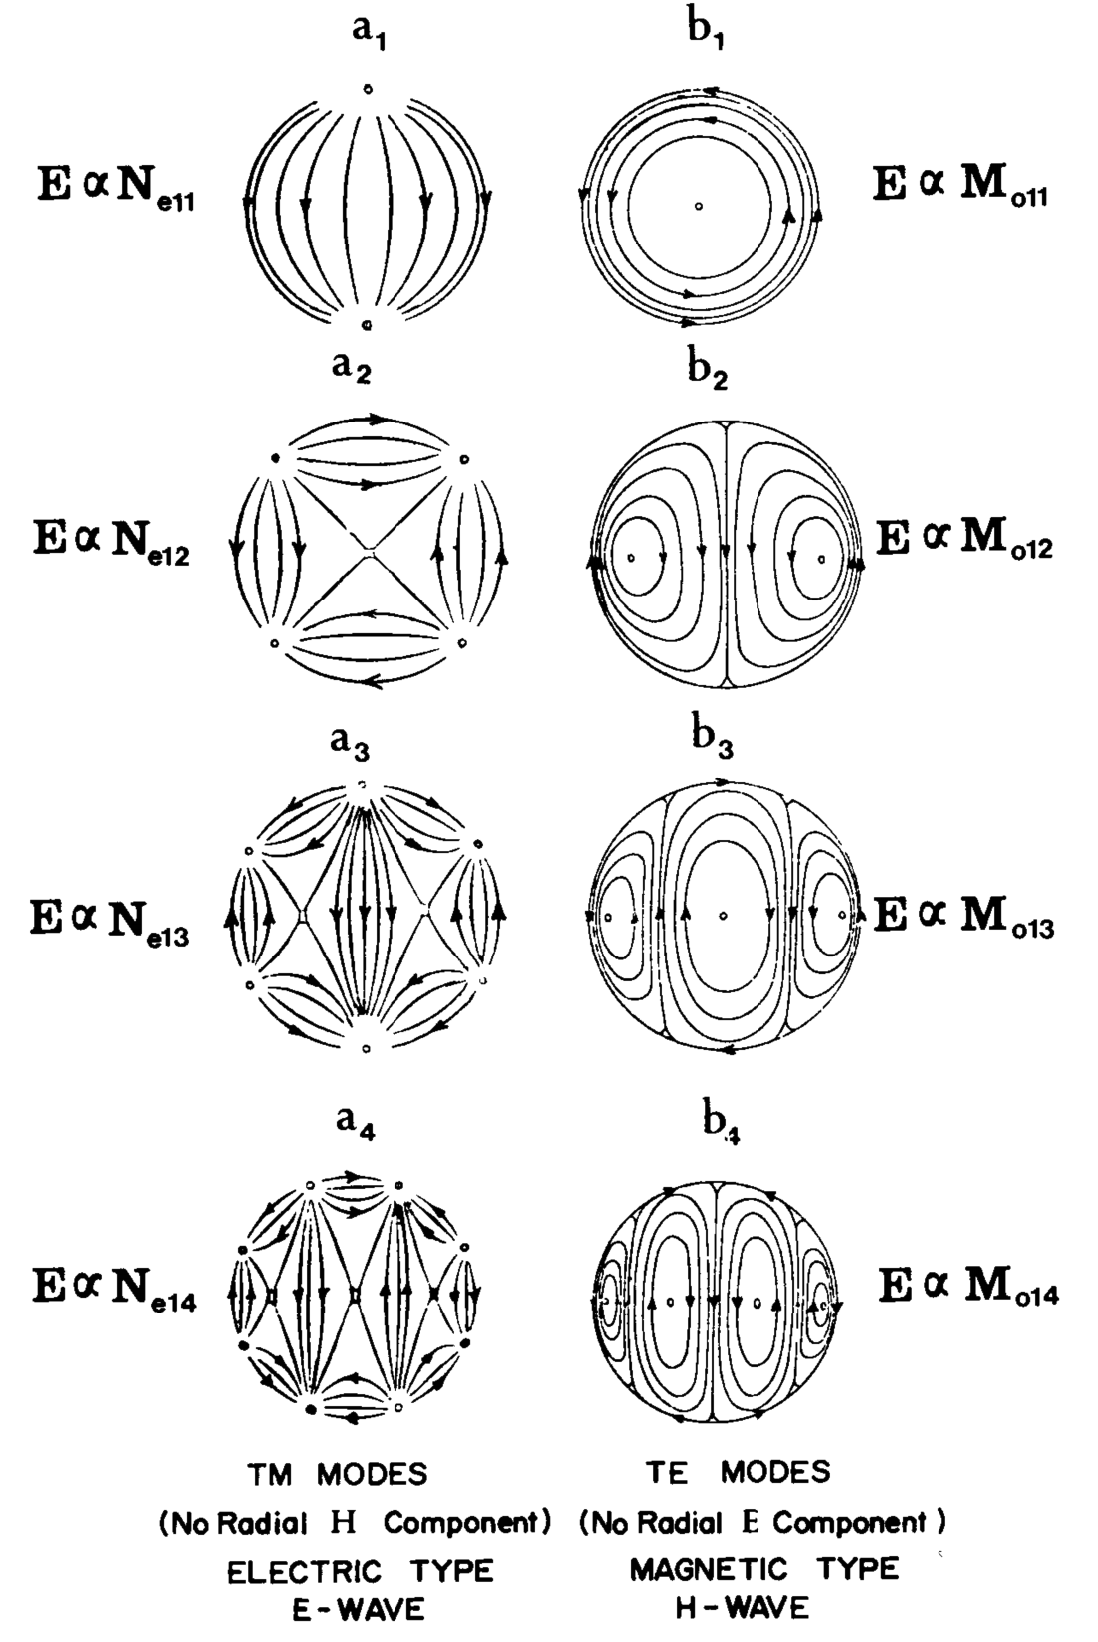
\includegraphics[width=.8\textwidth]{img/Mie_total}
			\caption{\bibentry{Bohren1998}}
		\end{figure}
	\end{minipage}%
	\begin{minipage}[t][\textheight]{.5\textwidth}
		\begin{figure}
			\centering
			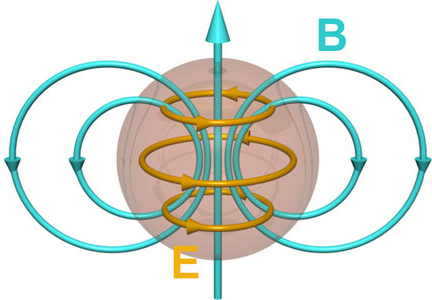
\includegraphics[width=\textwidth]{img/mie_reson}
			\caption{\bibentry{Kuznetsov2012}}
		\end{figure}

		\begin{itemize}
			\item Сферы, позже цилиндры
			\item Первая магнитная мода
			\item Ненулевой магнитный дипольный момент	
		\end{itemize}
	\end{minipage}
\end{frame}
  	\begin{frame}{Сверхбыстрые полностью оптические переключатели}
	\begin{figure}
		\begin{subfigure}{.35\textwidth}
			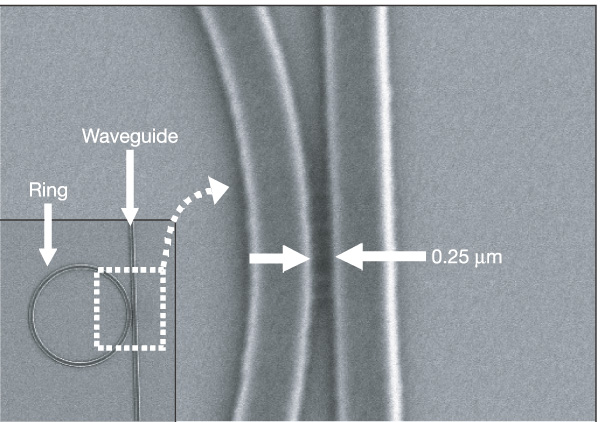
\includegraphics[width=.95\textwidth]{img/ring}
			\vspace{.5em}
			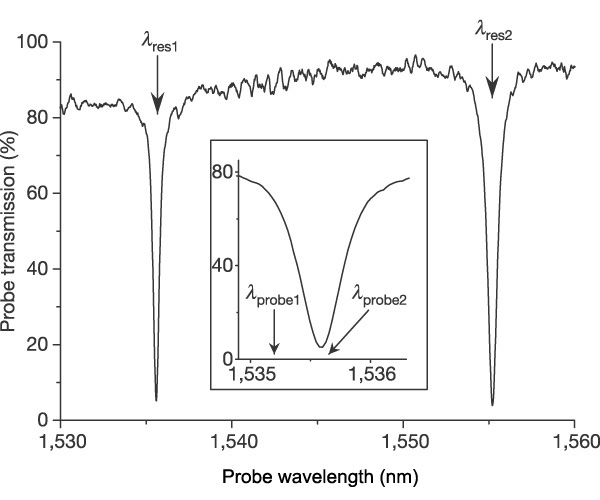
\includegraphics[width=.95\textwidth]{img/ring_spectrum}
		\end{subfigure}%
		\begin{subfigure}{.65\textwidth}
			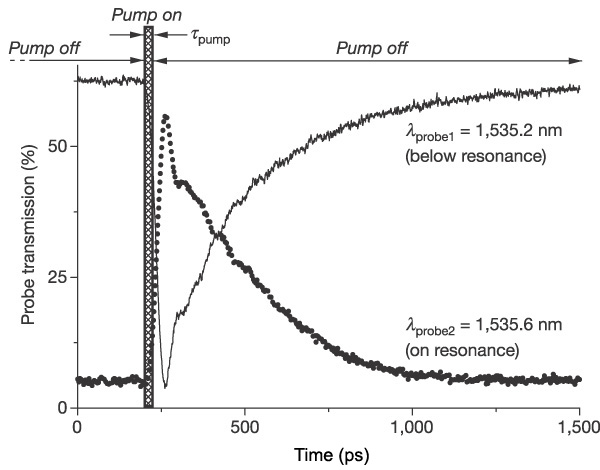
\includegraphics[width=\textwidth]{img/ring_res_shift}
		\end{subfigure}
		\caption{\bibentry{Vilson2004}}
	\end{figure}%
	\begin{itemize}
		\item Изменение показателя преломления путём двухфотонного поглощения
	\end{itemize}
\end{frame}
  	\begin{frame}{Исследуемые наноструктуры}
	\begin{minipage}[b]{.5\textwidth}
		
\includegraphics[width=.95\textwidth]{img/scheme_yz3}
		
		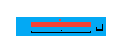
\includegraphics[width=.9\textwidth]{img/scheme_xy3}
		\vspace{3em}
	\end{minipage}%
	\begin{minipage}[b]{.5\textwidth}
		\begin{table}
			\begin{tabular}{|c|c|}
				\hline
				Параметр & Значение\\
				\hline
				\hline
				$\lambda$ & 1.0 мкм--2.0 мкм \\
				\hline
				$L$ & 10 мкм \\
				\hline
				$w$ & 0.6 мкм \\
				\hline
				$h$ & 0.25 мкм, 0.4 мкм \\
				\hline
				$r$ & 0.1 мкм--1.0 мкм\\
				\hline
				$d$ & $-$0.09 мкм--1.0 мкм\\
				\hline
				$N$ & 1--20 \\
				\hline
				$D_{i, i+1}$ & 0 мкм--0.4 мкм \\
				\hline
			\end{tabular}
		\end{table}
	\end{minipage}
	
	
\includegraphics[width=\textwidth]{img/scheme_xz}
\end{frame}
  
  	\begin{frame}
  		\bibliographystyle{presentation}
		\bibliography{literature-abbrv}
  	\end{frame}
\end{document}